\subsection{Powering the Display}
\begin{figure*}
\onecolumn
\setcounter{problem}{6}  
%%%%%%%%%%%%%%%%%%%%%%%%%%%%%%%%%%%%%%%%%%%%%%%%%%%%%%%%%%%%%%%%%%%%%%
%%                                                                  %%
%%  This is the header of a LaTeX2e file exported from Gnumeric.    %%
%%                                                                  %%
%%  This file can be compiled as it stands or included in another   %%
%%  LaTeX document. The table is based on the longtable package so  %%
%%  the longtable options (headers, footers...) can be set in the   %%
%%  preamble section below (see PRAMBLE).                           %%
%%                                                                  %%
%%  To include the file in another, the following two lines must be %%
%%  in the including file:                                          %%
%%        \def\inputGnumericTable{}                                 %%
%%  at the beginning of the file and:                               %%
%%        \input{name-of-this-file.tex}                             %%
%%  where the table is to be placed. Note also that the including   %%
%%  file must use the following packages for the table to be        %%
%%  rendered correctly:                                             %%
%%    \usepackage[latin1]{inputenc}                                 %%
%%    \usepackage{color}                                            %%
%%    \usepackage{array}                                            %%
%%    \usepackage{longtable}                                        %%
%%    \usepackage{calc}                                             %%
%%    \usepackage{multirow}                                         %%
%%    \usepackage{hhline}                                           %%
%%    \usepackage{ifthen}                                           %%
%%  optionally (for landscape tables embedded in another document): %%
%%    \usepackage{lscape}                                           %%
%%                                                                  %%
%%%%%%%%%%%%%%%%%%%%%%%%%%%%%%%%%%%%%%%%%%%%%%%%%%%%%%%%%%%%%%%%%%%%%%



%%  This section checks if we are begin input into another file or  %%
%%  the file will be compiled alone. First use a macro taken from   %%
%%  the TeXbook ex 7.7 (suggestion of Han-Wen Nienhuys).            %%
\def\ifundefined#1{\expandafter\ifx\csname#1\endcsname\relax}


%%  Check for the \def token for inputed files. If it is not        %%
%%  defined, the file will be processed as a standalone and the     %%
%%  preamble will be used.                                          %%
\ifundefined{inputGnumericTable}

%%  We must be able to close or not the document at the end.        %%
	\def\gnumericTableEnd{\end{document}}


%%%%%%%%%%%%%%%%%%%%%%%%%%%%%%%%%%%%%%%%%%%%%%%%%%%%%%%%%%%%%%%%%%%%%%
%%                                                                  %%
%%  This is the PREAMBLE. Change these values to get the right      %%
%%  paper size and other niceties.                                  %%
%%                                                                  %%
%%%%%%%%%%%%%%%%%%%%%%%%%%%%%%%%%%%%%%%%%%%%%%%%%%%%%%%%%%%%%%%%%%%%%%

	%\documentclass[12pt%
			  %%,landscape%
                    %]{report}
       %\usepackage[latin1]{inputenc}
       %\usepackage{fullpage}
       %\usepackage{color}
       %\usepackage{array}
       %\usepackage{longtable}
       %\usepackage{calc}
       %\usepackage{multirow}
       %\usepackage{hhline}
       %\usepackage{ifthen}

	\begin{document}


%%  End of the preamble for the standalone. The next section is for %%
%%  documents which are included into other LaTeX2e files.          %%
\else

%%  We are not a stand alone document. For a regular table, we will %%
%%  have no preamble and only define the closing to mean nothing.   %%
    \def\gnumericTableEnd{}

%%  If we want landscape mode in an embedded document, comment out  %%
%%  the line above and uncomment the two below. The table will      %%
%%  begin on a new page and run in landscape mode.                  %%
%       \def\gnumericTableEnd{\end{landscape}}
%       \begin{landscape}


%%  End of the else clause for this file being \input.              %%
\fi

%%%%%%%%%%%%%%%%%%%%%%%%%%%%%%%%%%%%%%%%%%%%%%%%%%%%%%%%%%%%%%%%%%%%%%
%%                                                                  %%
%%  The rest is the gnumeric table, except for the closing          %%
%%  statement. Changes below will alter the table's appearance.     %%
%%                                                                  %%
%%%%%%%%%%%%%%%%%%%%%%%%%%%%%%%%%%%%%%%%%%%%%%%%%%%%%%%%%%%%%%%%%%%%%%

\providecommand{\gnumericmathit}[1]{#1} 
%%  Uncomment the next line if you would like your numbers to be in %%
%%  italics if they are italizised in the gnumeric table.           %%
%\renewcommand{\gnumericmathit}[1]{\mathit{#1}}
\providecommand{\gnumericPB}[1]%
{\let\gnumericTemp=\\#1\let\\=\gnumericTemp\hspace{0pt}}
 \ifundefined{gnumericTableWidthDefined}
        \newlength{\gnumericTableWidth}
        \newlength{\gnumericTableWidthComplete}
        \newlength{\gnumericMultiRowLength}
        \global\def\gnumericTableWidthDefined{}
 \fi
%% The following setting protects this code from babel shorthands.  %%
 \ifthenelse{\isundefined{\languageshorthands}}{}{\languageshorthands{english}}
%%  The default table format retains the relative column widths of  %%
%%  gnumeric. They can easily be changed to c, r or l. In that case %%
%%  you may want to comment out the next line and uncomment the one %%
%%  thereafter                                                      %%
\providecommand\gnumbox{\makebox[0pt]}
%%\providecommand\gnumbox[1][]{\makebox}

%% to adjust positions in multirow situations                       %%
\setlength{\bigstrutjot}{\jot}
\setlength{\extrarowheight}{\doublerulesep}

%%  The \setlongtables command keeps column widths the same across  %%
%%  pages. Simply comment out next line for varying column widths.  %%
\setlongtables

\setlength\gnumericTableWidth{%
	50pt+%
	71pt+%
	50pt+%
	50pt+%
	50pt+%
	50pt+%
	50pt+%
	50pt+%
0pt}
\def\gumericNumCols{8}
\setlength\gnumericTableWidthComplete{\gnumericTableWidth+%
         \tabcolsep*\gumericNumCols*2+\arrayrulewidth*\gumericNumCols}
\ifthenelse{\lengthtest{\gnumericTableWidthComplete > \linewidth}}%
         {\def\gnumericScale{\ratio{\linewidth-%
                        \tabcolsep*\gumericNumCols*2-%
                        \arrayrulewidth*\gumericNumCols}%
{\gnumericTableWidth}}}%
{\def\gnumericScale{1}}

%%%%%%%%%%%%%%%%%%%%%%%%%%%%%%%%%%%%%%%%%%%%%%%%%%%%%%%%%%%%%%%%%%%%%%
%%                                                                  %%
%% The following are the widths of the various columns. We are      %%
%% defining them here because then they are easier to change.       %%
%% Depending on the cell formats we may use them more than once.    %%
%%                                                                  %%
%%%%%%%%%%%%%%%%%%%%%%%%%%%%%%%%%%%%%%%%%%%%%%%%%%%%%%%%%%%%%%%%%%%%%%

\ifthenelse{\isundefined{\gnumericColA}}{\newlength{\gnumericColA}}{}\settowidth{\gnumericColA}{\begin{tabular}{@{}p{50pt*\gnumericScale}@{}}x\end{tabular}}
\ifthenelse{\isundefined{\gnumericColB}}{\newlength{\gnumericColB}}{}\settowidth{\gnumericColB}{\begin{tabular}{@{}p{71pt*\gnumericScale}@{}}x\end{tabular}}
\ifthenelse{\isundefined{\gnumericColC}}{\newlength{\gnumericColC}}{}\settowidth{\gnumericColC}{\begin{tabular}{@{}p{50pt*\gnumericScale}@{}}x\end{tabular}}
\ifthenelse{\isundefined{\gnumericColD}}{\newlength{\gnumericColD}}{}\settowidth{\gnumericColD}{\begin{tabular}{@{}p{50pt*\gnumericScale}@{}}x\end{tabular}}
\ifthenelse{\isundefined{\gnumericColE}}{\newlength{\gnumericColE}}{}\settowidth{\gnumericColE}{\begin{tabular}{@{}p{50pt*\gnumericScale}@{}}x\end{tabular}}
\ifthenelse{\isundefined{\gnumericColF}}{\newlength{\gnumericColF}}{}\settowidth{\gnumericColF}{\begin{tabular}{@{}p{50pt*\gnumericScale}@{}}x\end{tabular}}
\ifthenelse{\isundefined{\gnumericColG}}{\newlength{\gnumericColG}}{}\settowidth{\gnumericColG}{\begin{tabular}{@{}p{50pt*\gnumericScale}@{}}x\end{tabular}}
\ifthenelse{\isundefined{\gnumericColH}}{\newlength{\gnumericColH}}{}\settowidth{\gnumericColH}{\begin{tabular}{@{}p{50pt*\gnumericScale}@{}}x\end{tabular}}

\begin{longtable}[c]{%
	b{\gnumericColA}%
	b{\gnumericColB}%
	b{\gnumericColC}%
	b{\gnumericColD}%
	b{\gnumericColE}%
	b{\gnumericColF}%
	b{\gnumericColG}%
	b{\gnumericColH}%
	}

%%%%%%%%%%%%%%%%%%%%%%%%%%%%%%%%%%%%%%%%%%%%%%%%%%%%%%%%%%%%%%%%%%%%%%
%%  The longtable options. (Caption, headers... see Goosens, p.124) %%
	\caption{Seven segment display to decimal.}             
	\label{table_1_6}
	\\	%
 \hline	% Across the top of the table.
%%  The rest of these options are table rows which are placed on    %%
%%  the first, last or every page. Use \multicolumn if you want.    %%

%%  Header for the first page.                                      %%
%	\multicolumn{8}{c}{The First Header} \\ \hline 
%	\multicolumn{1}{c}{colTag}	%Column 1
%	&\multicolumn{1}{c}{colTag}	%Column 2
%	&\multicolumn{1}{c}{colTag}	%Column 3
%	&\multicolumn{1}{c}{colTag}	%Column 4
%	&\multicolumn{1}{c}{colTag}	%Column 5
%	&\multicolumn{1}{c}{colTag}	%Column 6
%	&\multicolumn{1}{c}{colTag}	%Column 7
%	&\multicolumn{1}{c}{colTag}	\\ \hline %Last column
%	\endfirsthead

%%  The running header definition.                                  %%
%	\hline
%	\multicolumn{8}{l}{\ldots\small\slshape continued} \\ \hline
%	\multicolumn{1}{c}{colTag}	%Column 1
%	&\multicolumn{1}{c}{colTag}	%Column 2
%	&\multicolumn{1}{c}{colTag}	%Column 3
%	&\multicolumn{1}{c}{colTag}	%Column 4
%	&\multicolumn{1}{c}{colTag}	%Column 5
%	&\multicolumn{1}{c}{colTag}	%Column 6
%	&\multicolumn{1}{c}{colTag}	%Column 7
%	&\multicolumn{1}{c}{colTag}	\\ \hline %Last column
%	\endhead

%%  The running footer definition.                                  %%
%	\hline
%	\multicolumn{8}{r}{\small\slshape continued\ldots} \\
%	\endfoot

%%  The ending footer definition.                                   %%
%	\multicolumn{8}{c}{That's all folks} \\ \hline 
%	\endlastfoot
%%%%%%%%%%%%%%%%%%%%%%%%%%%%%%%%%%%%%%%%%%%%%%%%%%%%%%%%%%%%%%%%%%%%%%

\hhline{|-|-|-|-|-|-|-|-}
	 \multicolumn{1}{|p{\gnumericColA}|}%
	{\gnumericPB{\centering}\gnumbox{a}}
	&\multicolumn{1}{p{\gnumericColB}|}%
	{\gnumericPB{\centering}\gnumbox{b}}
	&\multicolumn{1}{p{\gnumericColC}|}%
	{\gnumericPB{\centering}\gnumbox{c}}
	&\multicolumn{1}{p{\gnumericColD}|}%
	{\gnumericPB{\centering}\gnumbox{d}}
	&\multicolumn{1}{p{\gnumericColE}|}%
	{\gnumericPB{\centering}\gnumbox{e}}
	&\multicolumn{1}{p{\gnumericColF}|}%
	{\gnumericPB{\centering}\gnumbox{f}}
	&\multicolumn{1}{p{\gnumericColG}|}%
	{\gnumericPB{\centering}\gnumbox{g}}
	&\multicolumn{1}{p{\gnumericColH}|}%
	{\gnumericPB{\centering}\gnumbox{decimal}}
\\
\hhline{|--------|}
	 \multicolumn{1}{|p{\gnumericColA}|}%
	{\gnumericPB{\centering}\gnumbox{1}}
	&\multicolumn{1}{p{\gnumericColB}|}%
	{\gnumericPB{\centering}\gnumbox{0}}
	&\multicolumn{1}{p{\gnumericColC}|}%
	{\gnumericPB{\centering}\gnumbox{0}}
	&\multicolumn{1}{p{\gnumericColD}|}%
	{\gnumericPB{\centering}\gnumbox{1}}
	&\multicolumn{1}{p{\gnumericColE}|}%
	{\gnumericPB{\centering}\gnumbox{1}}
	&\multicolumn{1}{p{\gnumericColF}|}%
	{\gnumericPB{\centering}\gnumbox{1}}
	&\multicolumn{1}{p{\gnumericColG}|}%
	{\gnumericPB{\centering}\gnumbox{1}}
	&\multicolumn{1}{p{\gnumericColH}|}%
	{\gnumericPB{\centering}\gnumbox{1}}
\\
\hhline{|-|-|-|-|-|-|-|-|}
\end{longtable}

\ifthenelse{\isundefined{\languageshorthands}}{}{\languageshorthands{\languagename}}
\gnumericTableEnd

%
\setcounter{problem}{0}  
\twocolumn
\end{figure*}

%
\begin{problem}
	Plug the display to the breadboard shown in Fig. \ref{fig_1_1}. The breadboard can be divided into 5 segments.  In each of the green segements, the pins are internally connected so as to have the same voltage.  Similarly, in the central segments, the pins in each column  are internally connected in the same fashion as the blue columns. 
%
\end{problem}
%
\begin{figure}[!ht]
\begin{center}
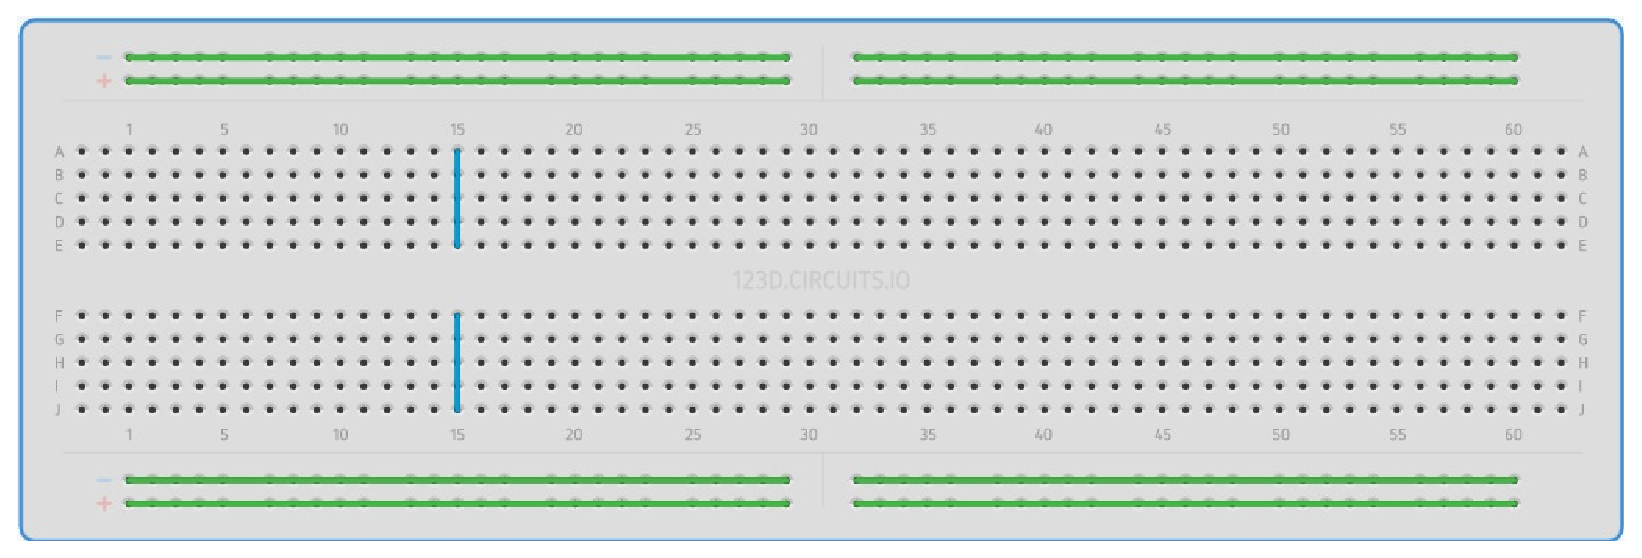
\includegraphics[width=\columnwidth]{./chapter1/figs/breadboard}
\end{center}
\captionof{figure}{Breadboard}
\label{fig_1_1}	
\end{figure}
%
\begin{problem}
	Connect one end of the 220 $\Omega$ resistor to the COM pin of the display in Fig. \ref{fig_1_2} and the other end to an extreme pin of the breadboard.	The seven segment display has eight pins, $a, b, c, d, e, f, g$ and $dot$ that take an active LOW input, i.e.  the LED will glow only if the input is connected to ground.  Each of these pins is connected to an LED segment.  The $dot$ pin is  reserved for the $\cdot$ LED.  
%
\end{problem}
%
\begin{figure}
\begin{center}
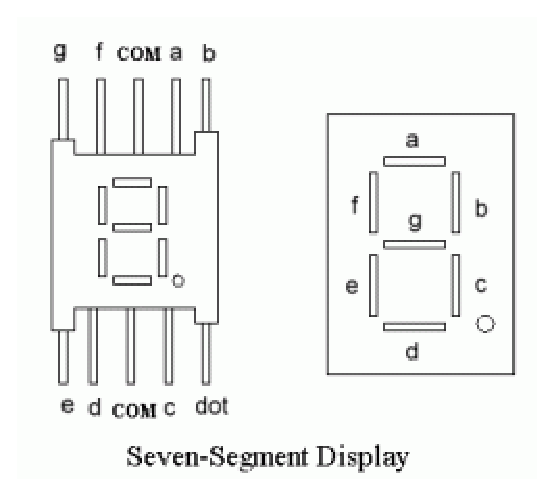
\includegraphics[width=\columnwidth]{./chapter1/figs/sevenseg}
\end{center}
\captionof{figure}{Seven Segment Display. }
\label{fig_1_2}
\end{figure}	%%
\begin{problem}
	Connect the 3.3$V$ pin of the Pi shown in Figs. \ref{fig_1_3a} and  \ref{fig_1_3b}  to an  extreme pin that is in the same segment as the 220 $\Omega$ resistor pin. 
\end{problem}	
\renewcommand{\thefigure}{\theproblem.\arabic{figure}}
\begin{figure}[!ht]
\begin{center}
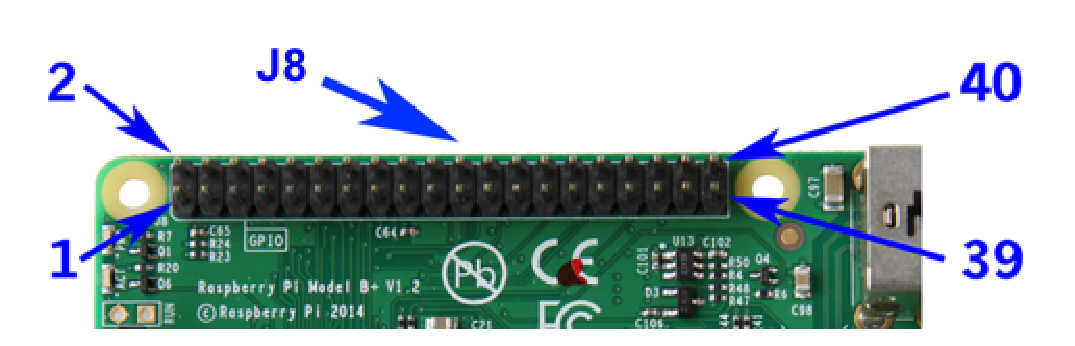
\includegraphics[width=\columnwidth]{./chapter1/figs/gpio2}
\end{center}
\captionof{figure}{GPIO pin snapshot on Pi \cite{gpio_pins}.}
\label{fig_1_3a}	
\end{figure}
%
\begin{figure}
\begin{center}
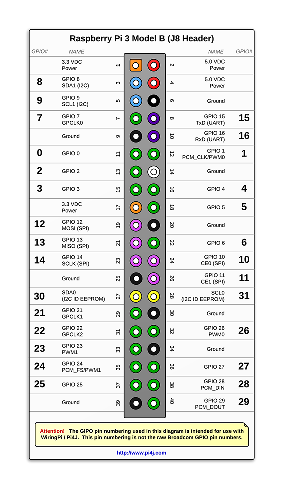
\includegraphics[width=\columnwidth]{./chapter1/figs/gpio1}
\end{center}
\captionof{figure}{GPIO Wiring Pi \cite{wiringpi} pin configuration.}
\label{fig_1_3b}	
\end{figure}
\renewcommand{\thefigure}{\theproblem}
%
\begin{problem}
	Connect the GND pin of the Pi to the opposite extreme pin of the breadboard
\end{problem}
\begin{problem}
	Connect the {\em dot} pin of the display to a pin in the same segment as the GND pin.  What do you observe?
\end{problem}
\subsection{Controlling the Display}
\begin{problem}
	Generate the number 1 on the display by connecting the pins $a-g$ to GND according to Table \ref{table_1_6}.
	\end{problem}
%
\begin{problem}
	Complete Table \ref{table_1_6} for all numbers between 0-9.
\end{problem}
%
\begin{problem}
	Now generate the numbers from 0-9 on the display using Table \ref{table_1_6}.
\end{problem}
%
\begin{problem}
	Connect the 7447 IC decoder $\bar{a}-\bar{g}$ pins  in Fig. \ref{fig_1_9} to the $a-g$ pins of the display respectively.
\end{problem}
%
\begin{figure}[!ht]
\begin{center}
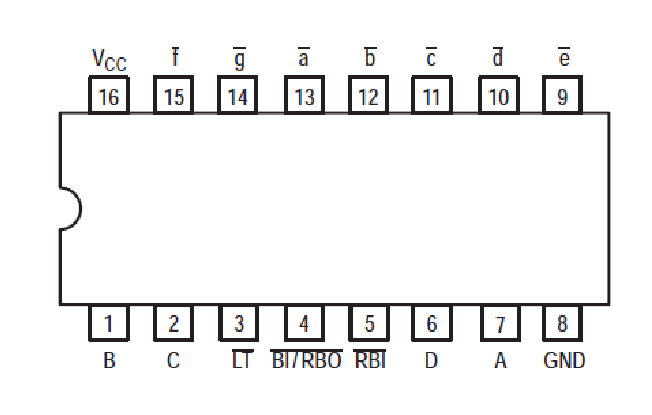
\includegraphics[width=\columnwidth]{./chapter1/figs/7447IC}
\end{center}
\captionof{figure}{7447 to seven segment display decoder.}
\label{fig_1_9}	
\end{figure}
%

\begin{problem}
	Connect the $V_{cc}$ and GND pins of the decoder in to the  supply and GND pins of the breadboard.
\end{problem}
\begin{problem}
	Connect the A,B,C,D pins in Fig. \ref{fig_1_9}  to pins in the GND extreme segment of the breadboard.  What do you observe?
\end{problem}
\begin{problem}
	Now remove the D pin from the breadboard and observe the display output.
\end{problem}
\begin{problem}
	Generate a table with A,B,C,D inputs and the equivalent decimal number output.
\end{problem}
The 7447 IC helps in displaying decimal numbers on the seven segment display.  The $\bar{a}-\bar{f}$, pins of the 7447 IC are connected to the $a-f$ pins of the display. $V_cc$ should be connected to a 5V power source. The input pins of the decoder are A,B,C and D, with A being the lowest significant bit (LSB) and D being the most significant bit (MSB).  For example, the number 5 is visible on the display when the A,B,C and D inputs are the following.
\begin{center}
	\begin{tabular}{|c|c|c|c|c|}
\hline
D & C & B & A & Decimal
\\ \hline
0 & 1 & 0 & 1 & 5
\\
\hline
\end{tabular}
\end{center}
